\documentclass{article}
\usepackage{amsfonts, amsmath, amssymb, amsthm} % Math notations imported
\usepackage[inline]{enumitem}
\usepackage{graphicx}
\usepackage{setspace}
\usepackage{indentfirst}
\usepackage[margin=1in]{geometry}
\graphicspath{{./images/}} % Path to images

% \begin{figure}[htb!]
%      \centering
%      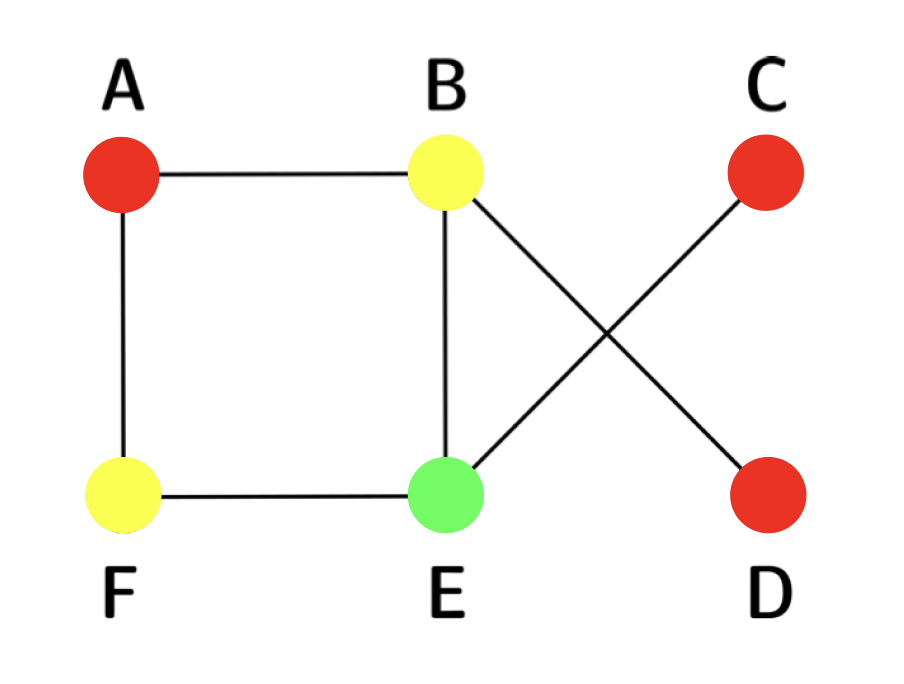
\includegraphics[scale=0.5]{coloring.png}
%      \caption{Coloring of the graph.}
% \end{figure}

% \begin{figure}[htb]
%     \qquad
%     \begin{minipage}{.4\textwidth}
%         \centering
%         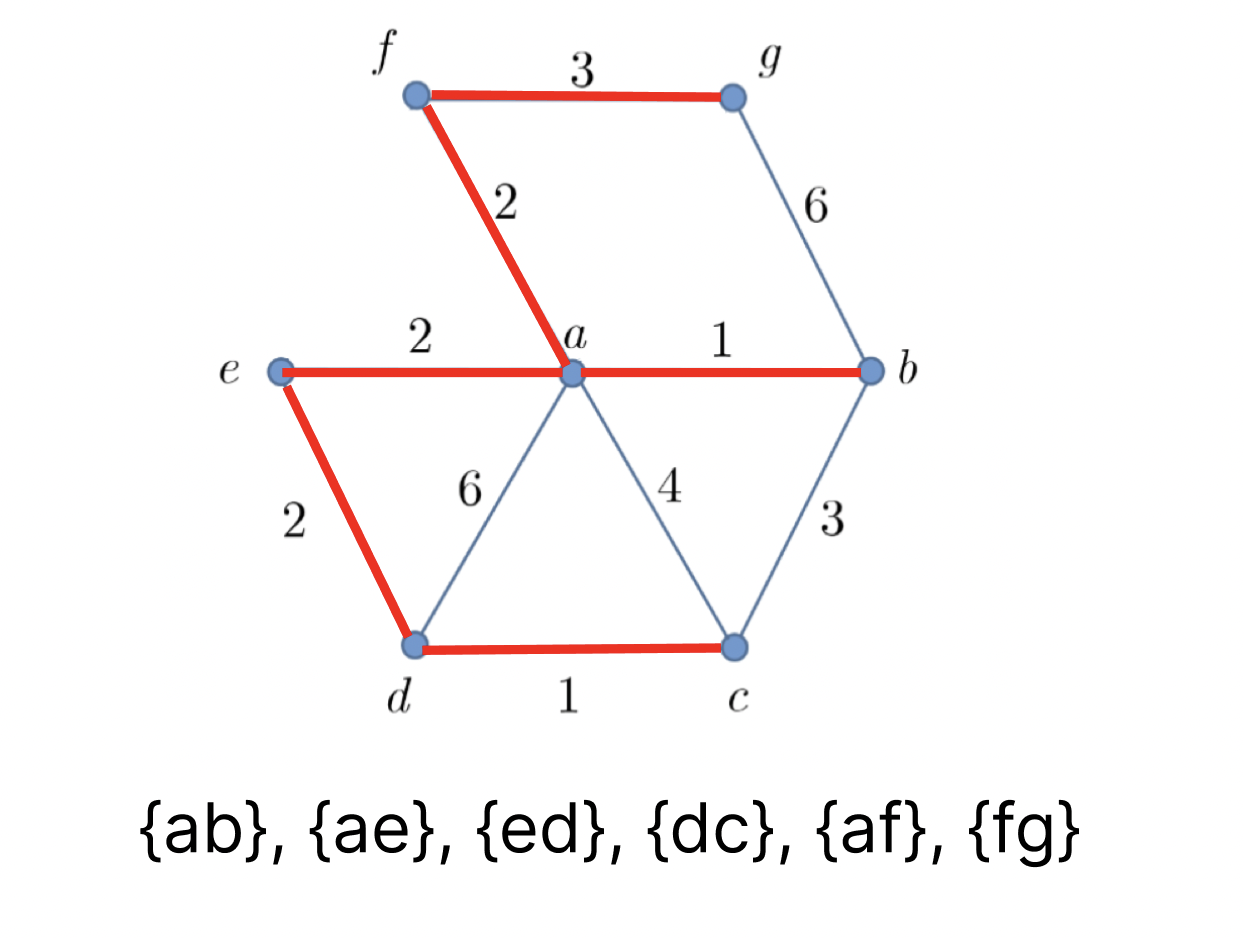
\includegraphics[scale=0.35]{prims.png}
%         \caption{}
%     \end{minipage}    
%     \qquad
%     \begin{minipage}{.4\textwidth}
%         \centering
%         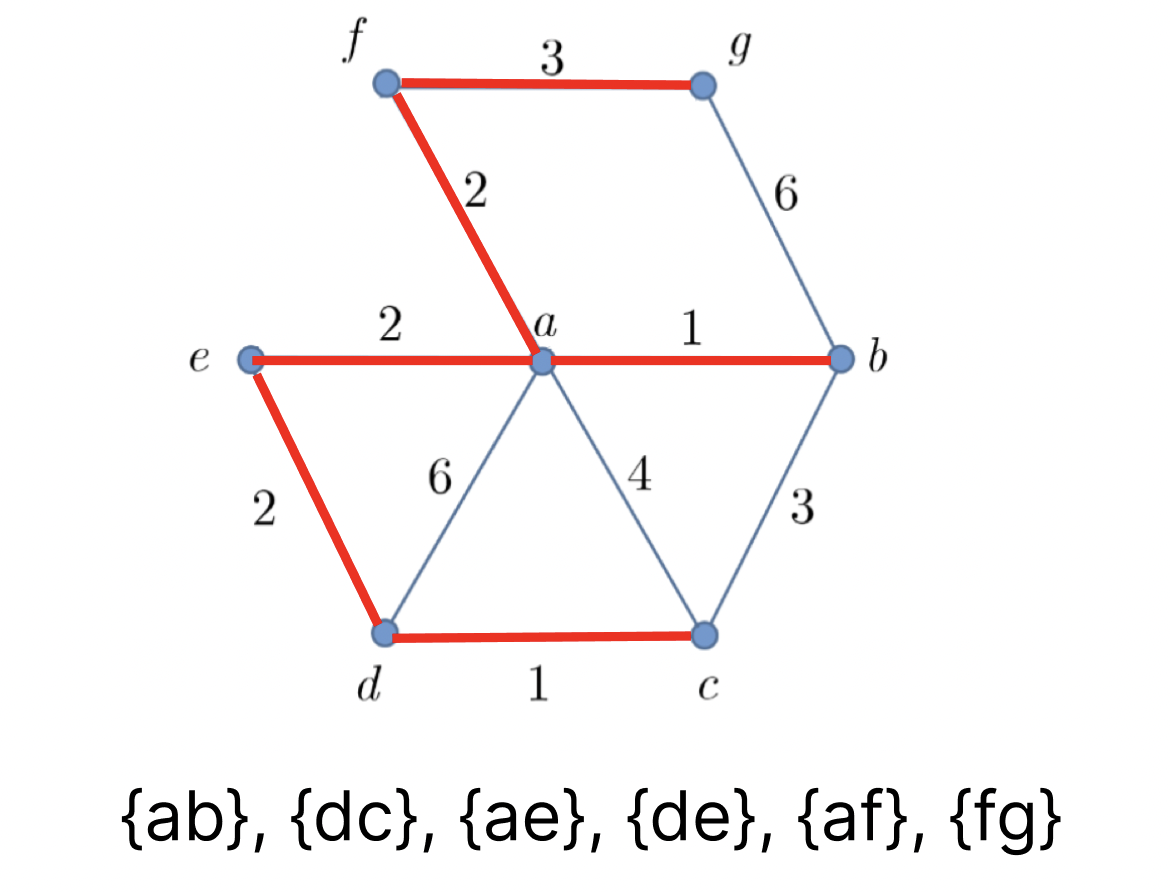
\includegraphics[scale=0.35]{kruskal.png}
%         \caption{}
%     \end{minipage}        
% \end{figure} 

\newtheorem{thm}{Theorem}
\newtheorem{proposition}[thm]{Proposition}
\newtheorem{cor}[thm]{Corollary}

% title information
\title{Math 128A HW3}
\author{Neo Lee}
\date{09/20/2023}

\setstretch{1.15}
% main content
\begin{document} 

% placing title information; comment out if using fancyhdr
\maketitle 

\section*{Section 2.5}
\subsection*{Problem 2}
Consider the function $f(x)=e^{6x}+3(ln2)^2e^{2x}-(ln8)e^{4x}-(ln2)^3$. Use Newton's method with 
$p_0=0$ to approximate a zero of $f$. Generate terms until $|p_{n+1}-p_n|<0.0002$. Construct the 
sequence $\{\hat{p}_n\}$. Is the convergence improved?
\begin{proof}[Solution]
    \begin{align*}
        f'(x) & = 6e^{6x}+6(ln2)^2e^{2x}-4(ln8)e^{4x} \\
        g(x) & = x-\frac{f(x)}{f'(x)} \\
        & = x-\frac{e^{6x}+3(ln2)^2e^{2x}-(ln8)e^{4x}-(ln2)^3}{6e^{6x}+6(ln2)^2e^{2x}-4(ln8)e^{4x}}.
    \end{align*}
    \begin{figure}[htb!]
        \centering
        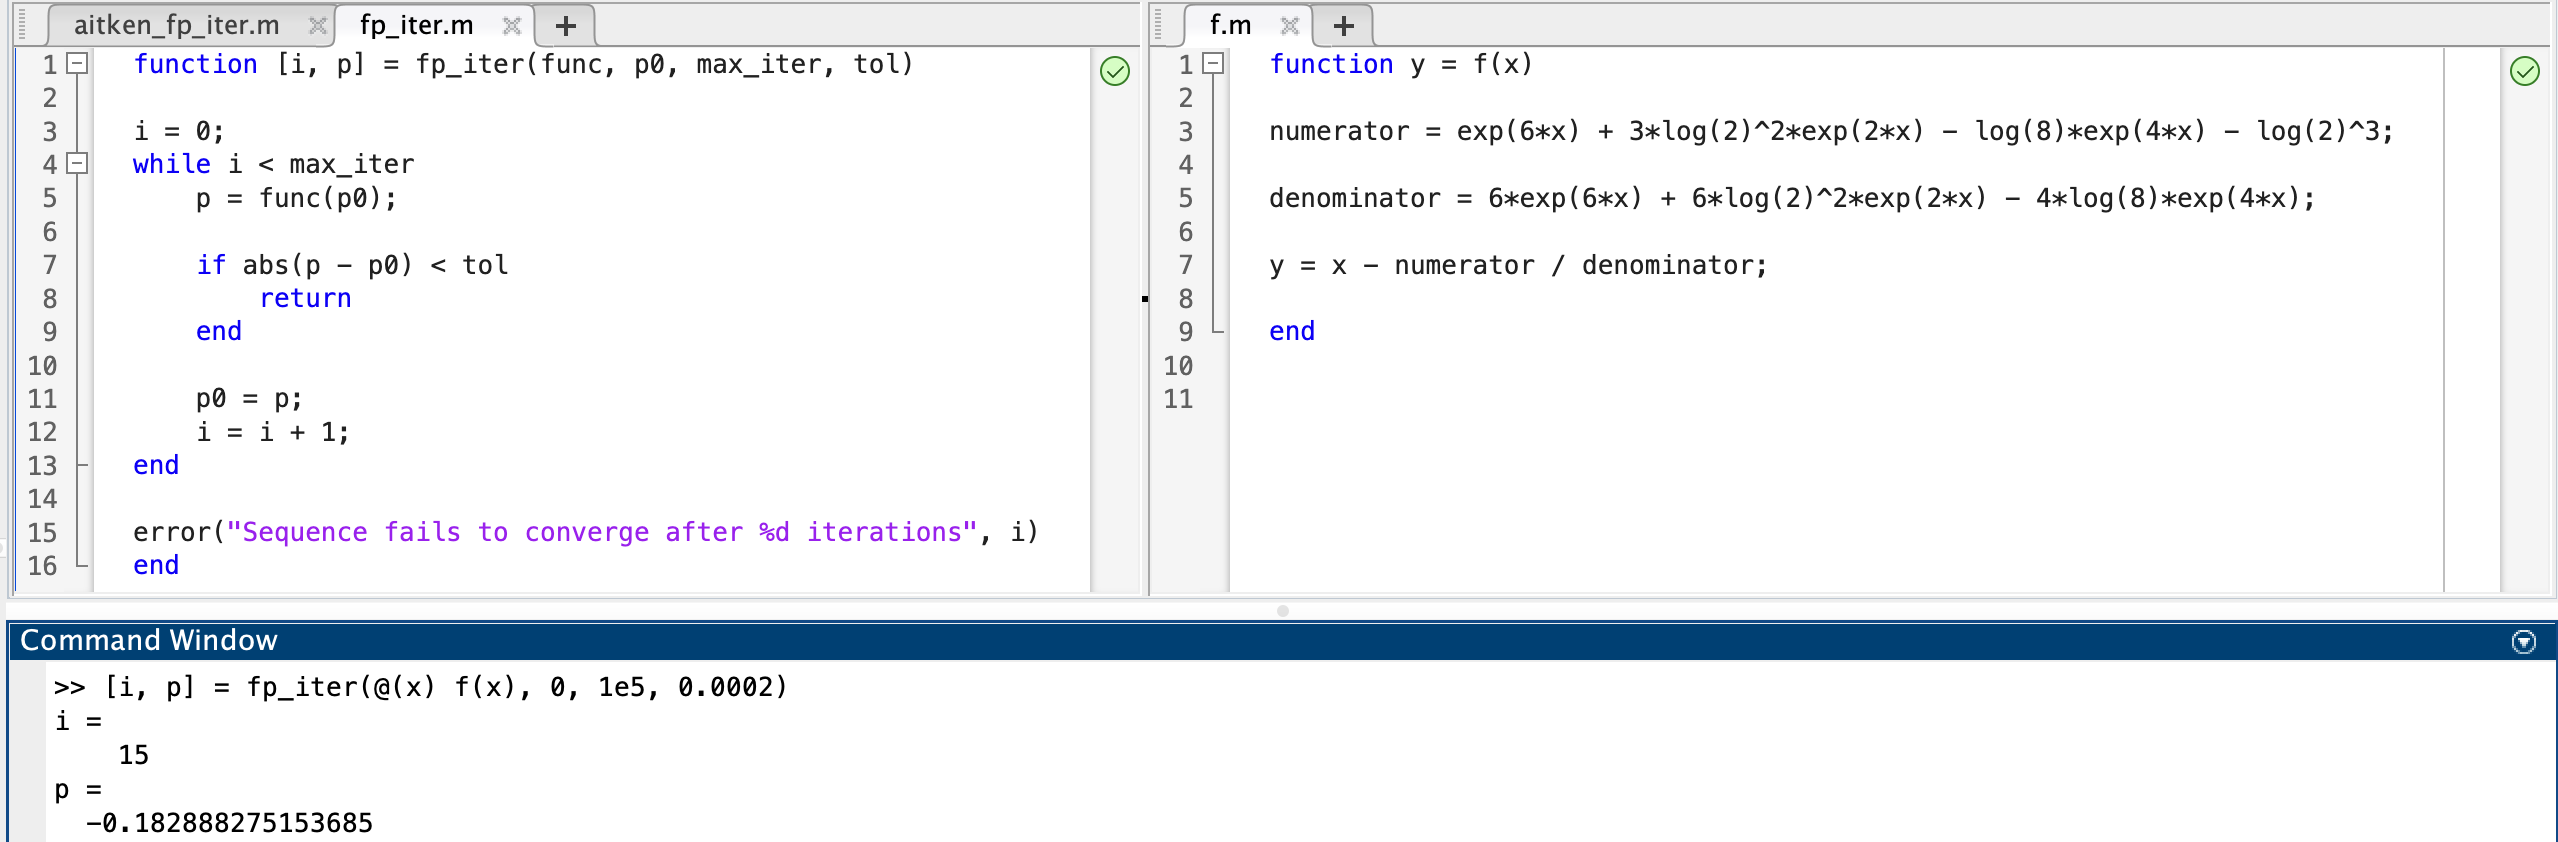
\includegraphics[scale=0.2]{2.5.2_1.png}
        \caption{Regular Newton's method: iteartions = 15}
    \end{figure}
    \begin{figure}[htb!]
        \centering
        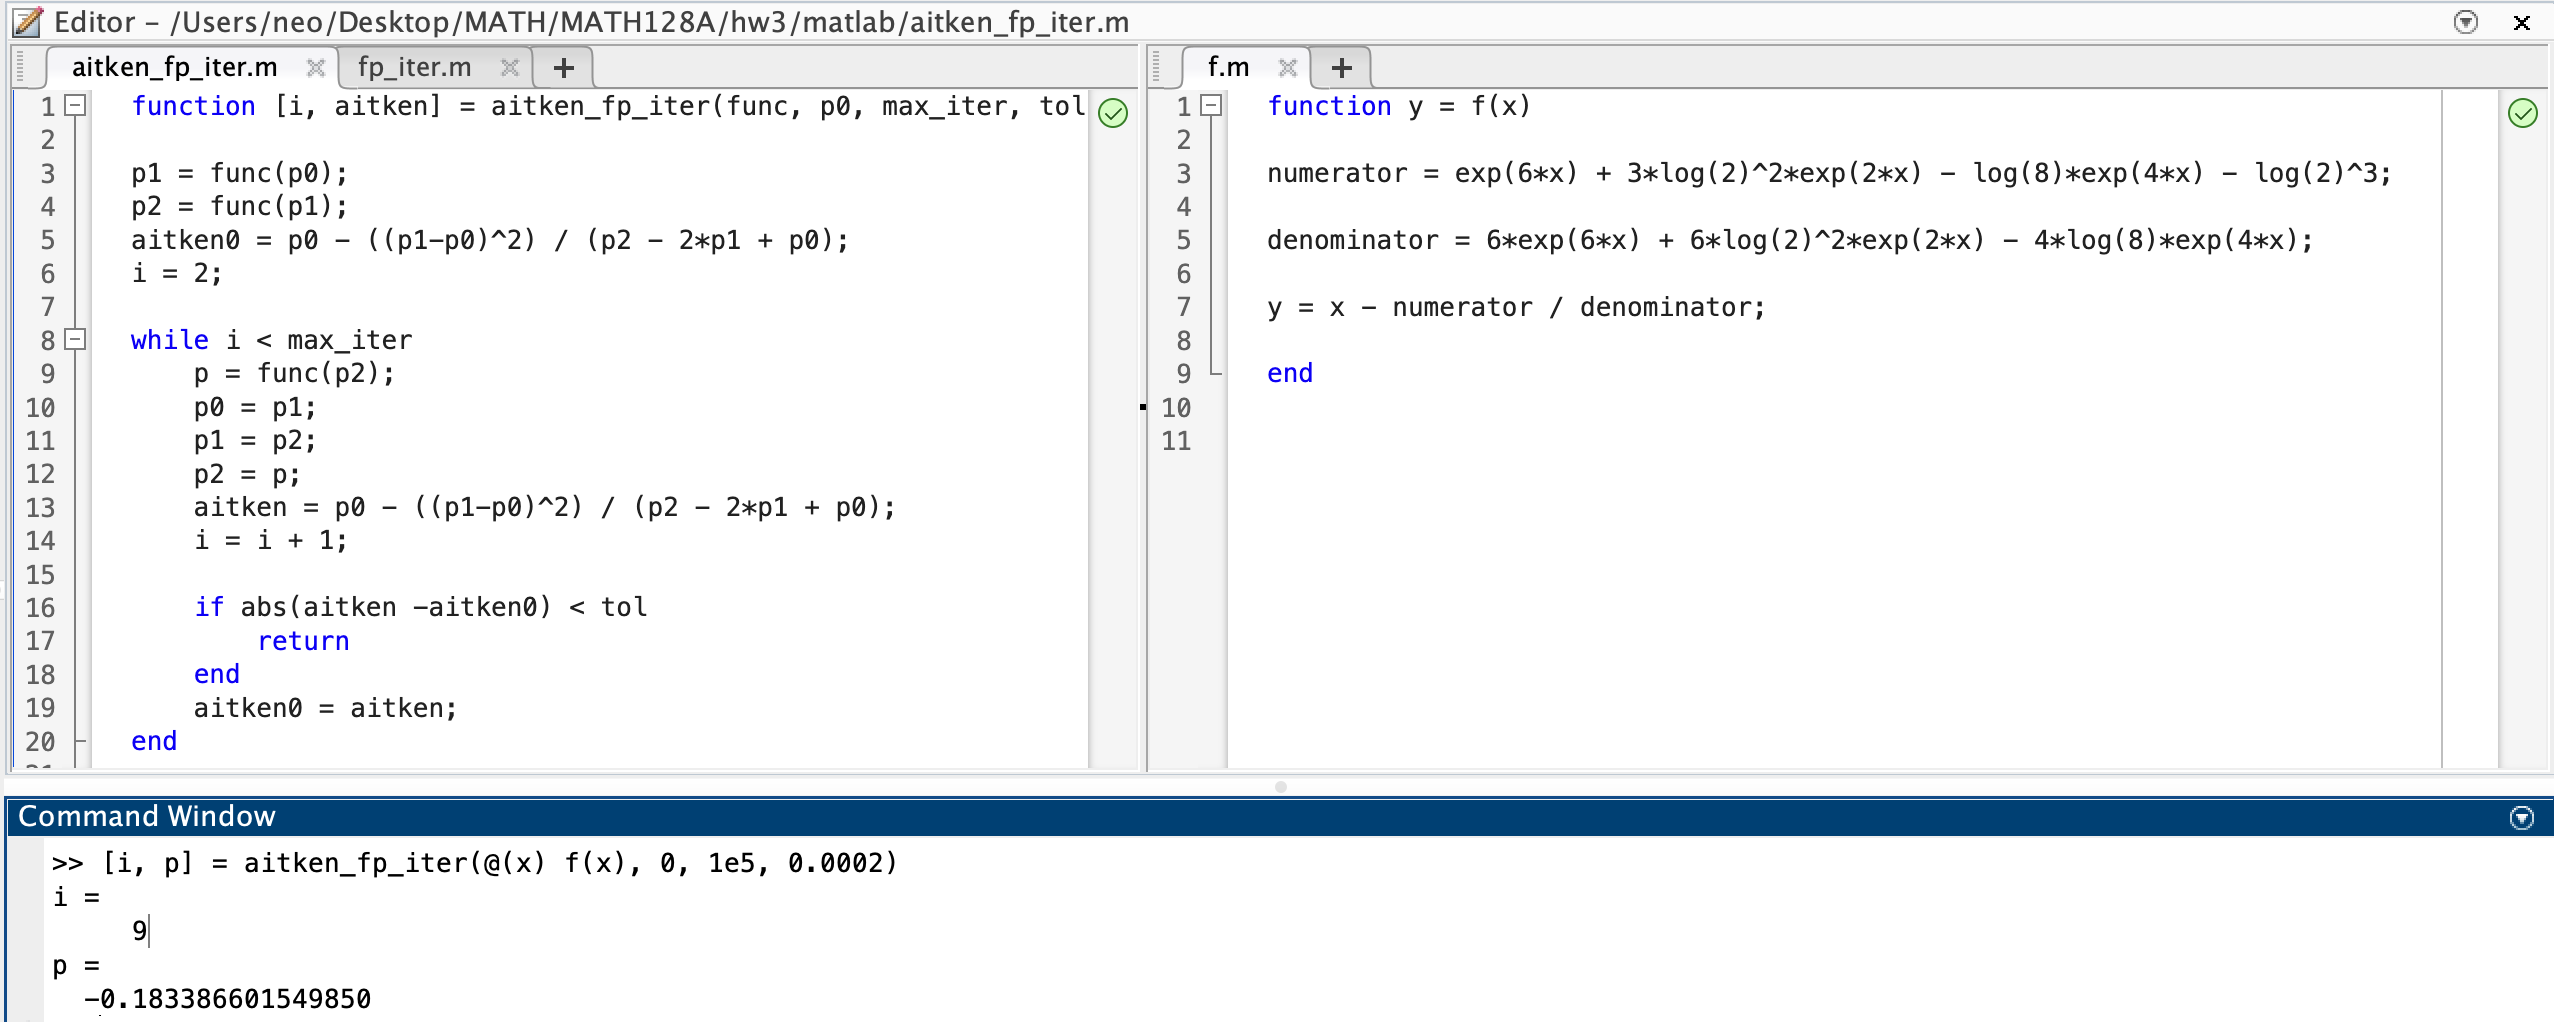
\includegraphics[scale=0.2]{2.5.2_2.png}
        \caption{Newtons' method with Aitken's $\Delta^2$ process: iterations = 9}
    \end{figure}
    
    The sequence converged with fewer iterations with Aitken's $\Delta^2$ process.
\end{proof}

\subsection*{Problem 4}
Let $g(x) = 1 + (sinx)^2$ and $p_0^{(0)} = 1$. Use Steffensen's method to find $p_0^{(1)}$ and 
$p_0^{(2)}$.
\begin{proof}[Solution]\indent
    \begin{figure}[htb!]
        \centering
        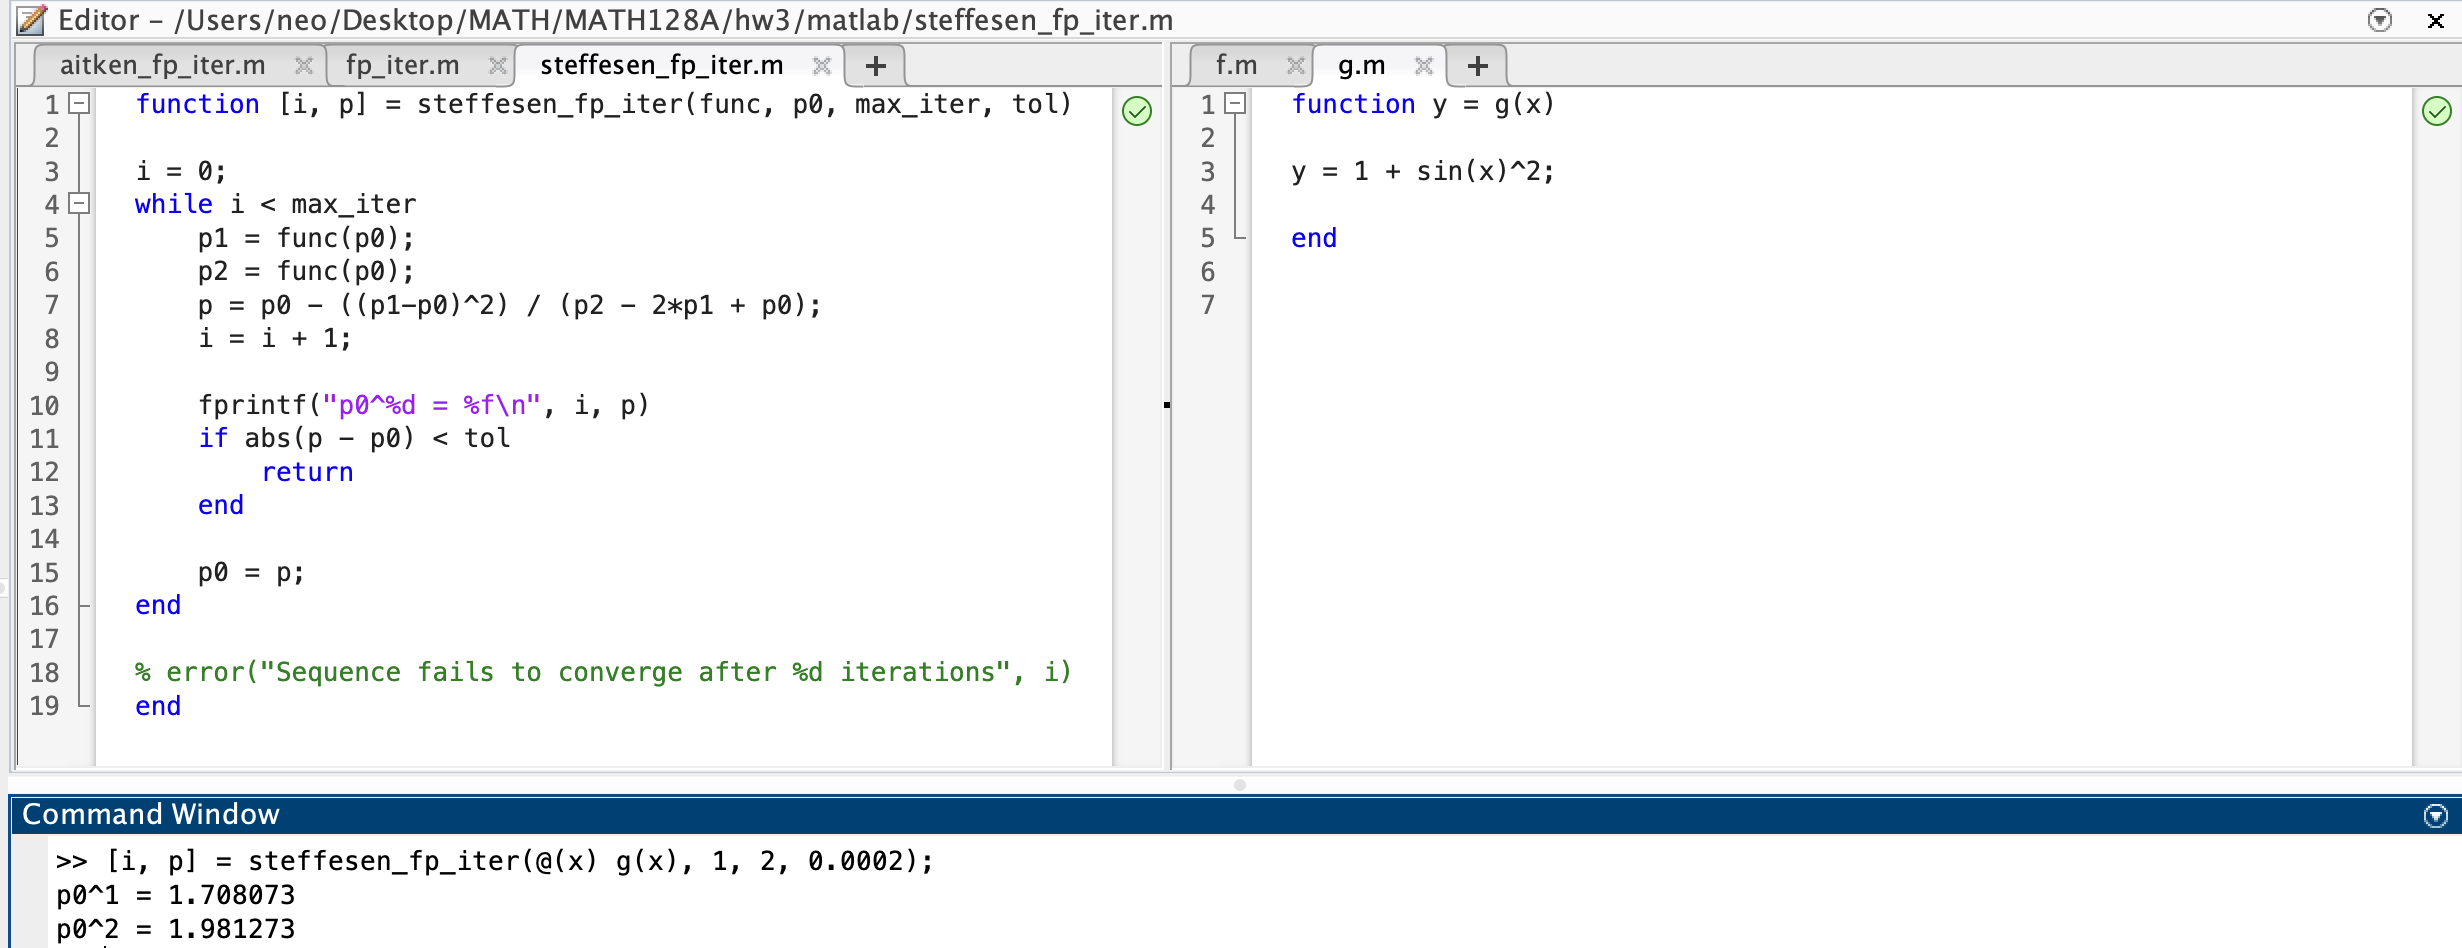
\includegraphics[scale=0.2]{2.5.4.png}
        \caption{$p_0^{(1)}=1.708, p_0^{(2)}=1.981$}
    \end{figure}
    
\end{proof}

\subsection*{Problem 7}
Use Steffensen's method to find, to an accuracy of $10^{-4}$, the root of $x^3-x-1=0$ that lies in 
$[1,2]$ and compare this to the results of Exercise 8 of Section 2.2.
\begin{proof}[Solution]
    Define $g(x):=(x+1)^{1/3}$ as our fixed-point iteration function and use $p_0=1$.
    \begin{figure}[htb!]
        \centering
        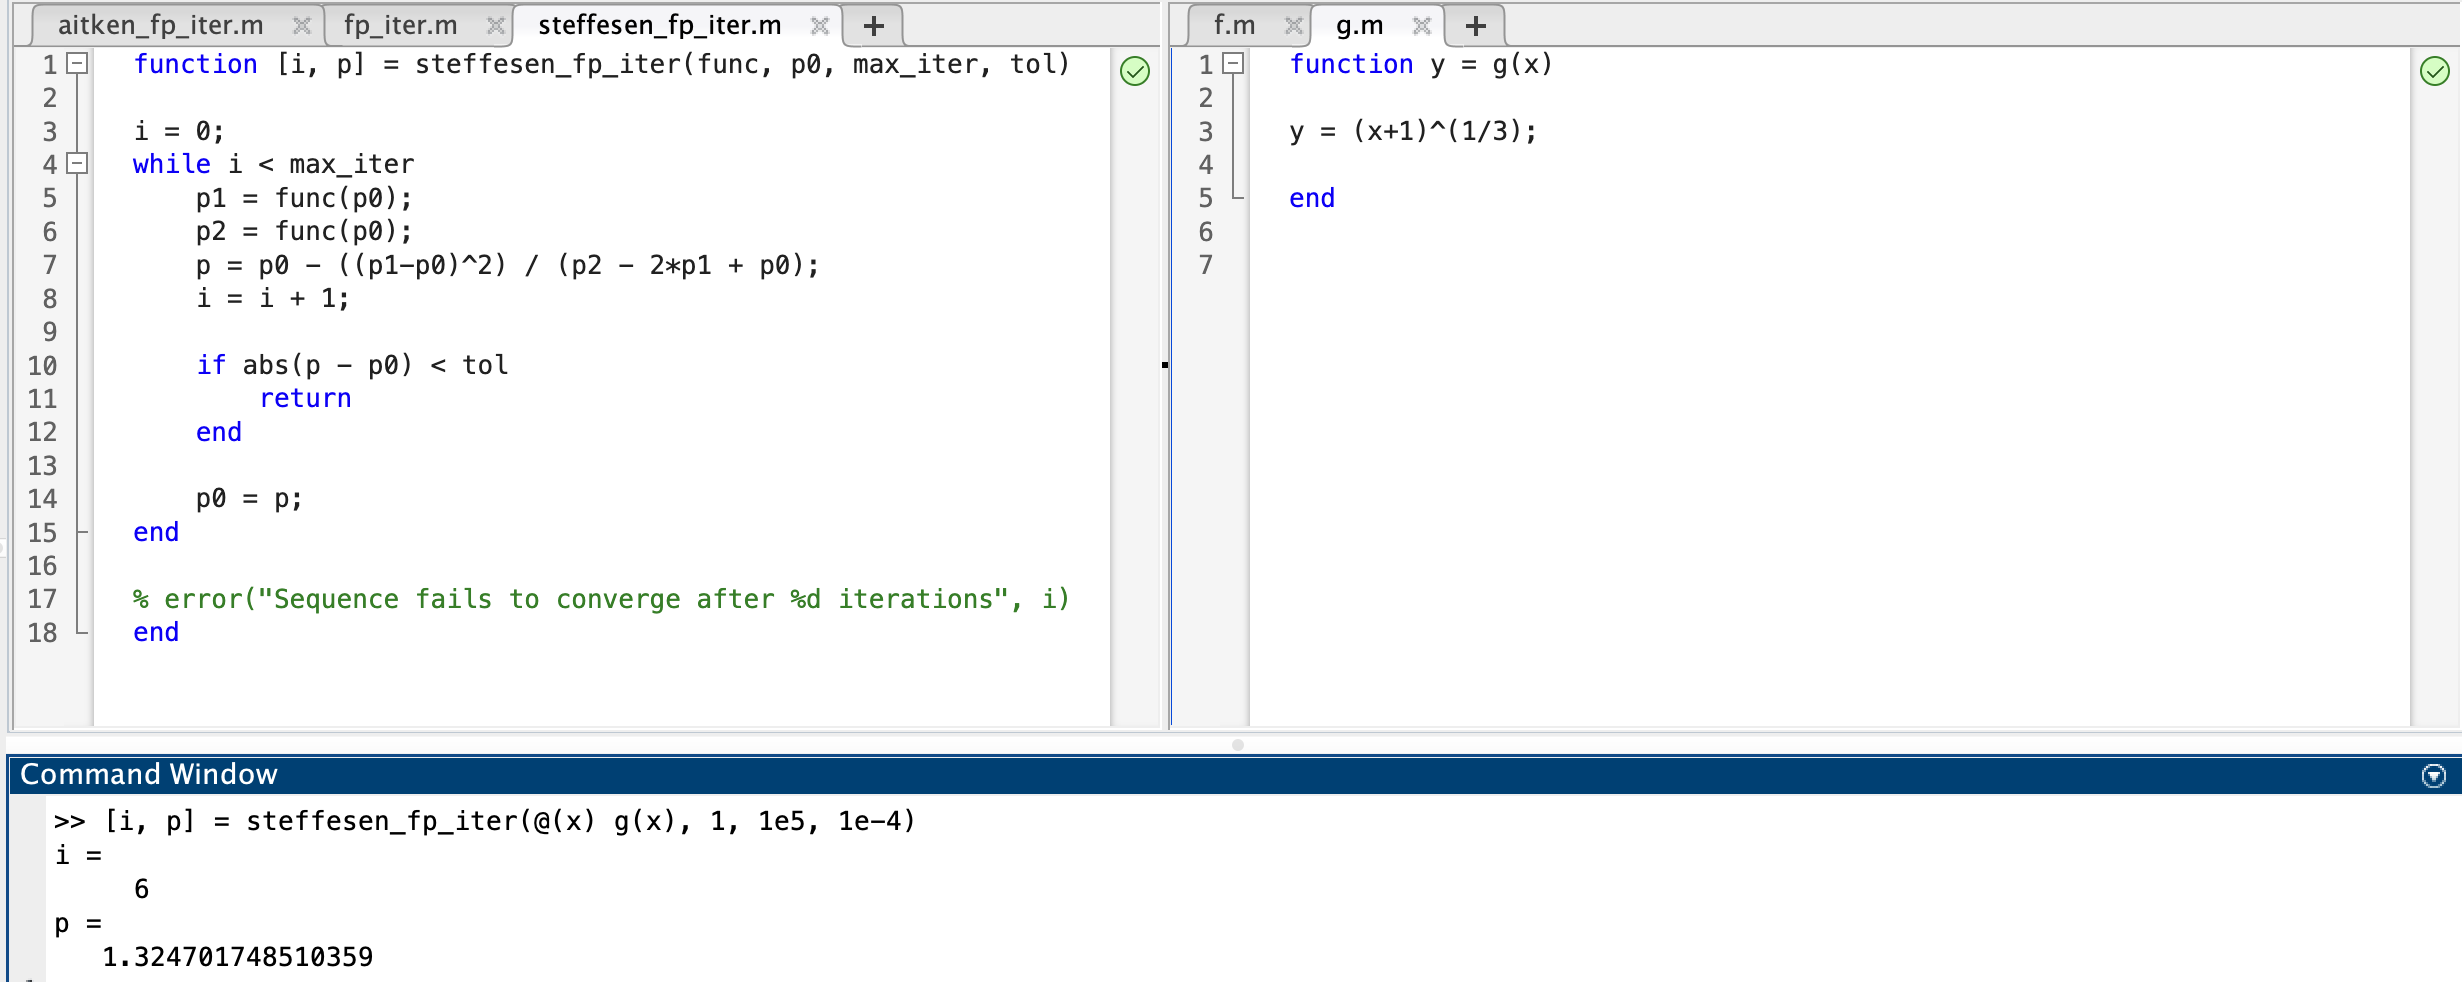
\includegraphics[scale=0.2]{2.5.7_1.png}
        \caption{$p = 1.3247$, iterations = 6}
    \end{figure}
    \begin{figure}[htb!]
        \centering
        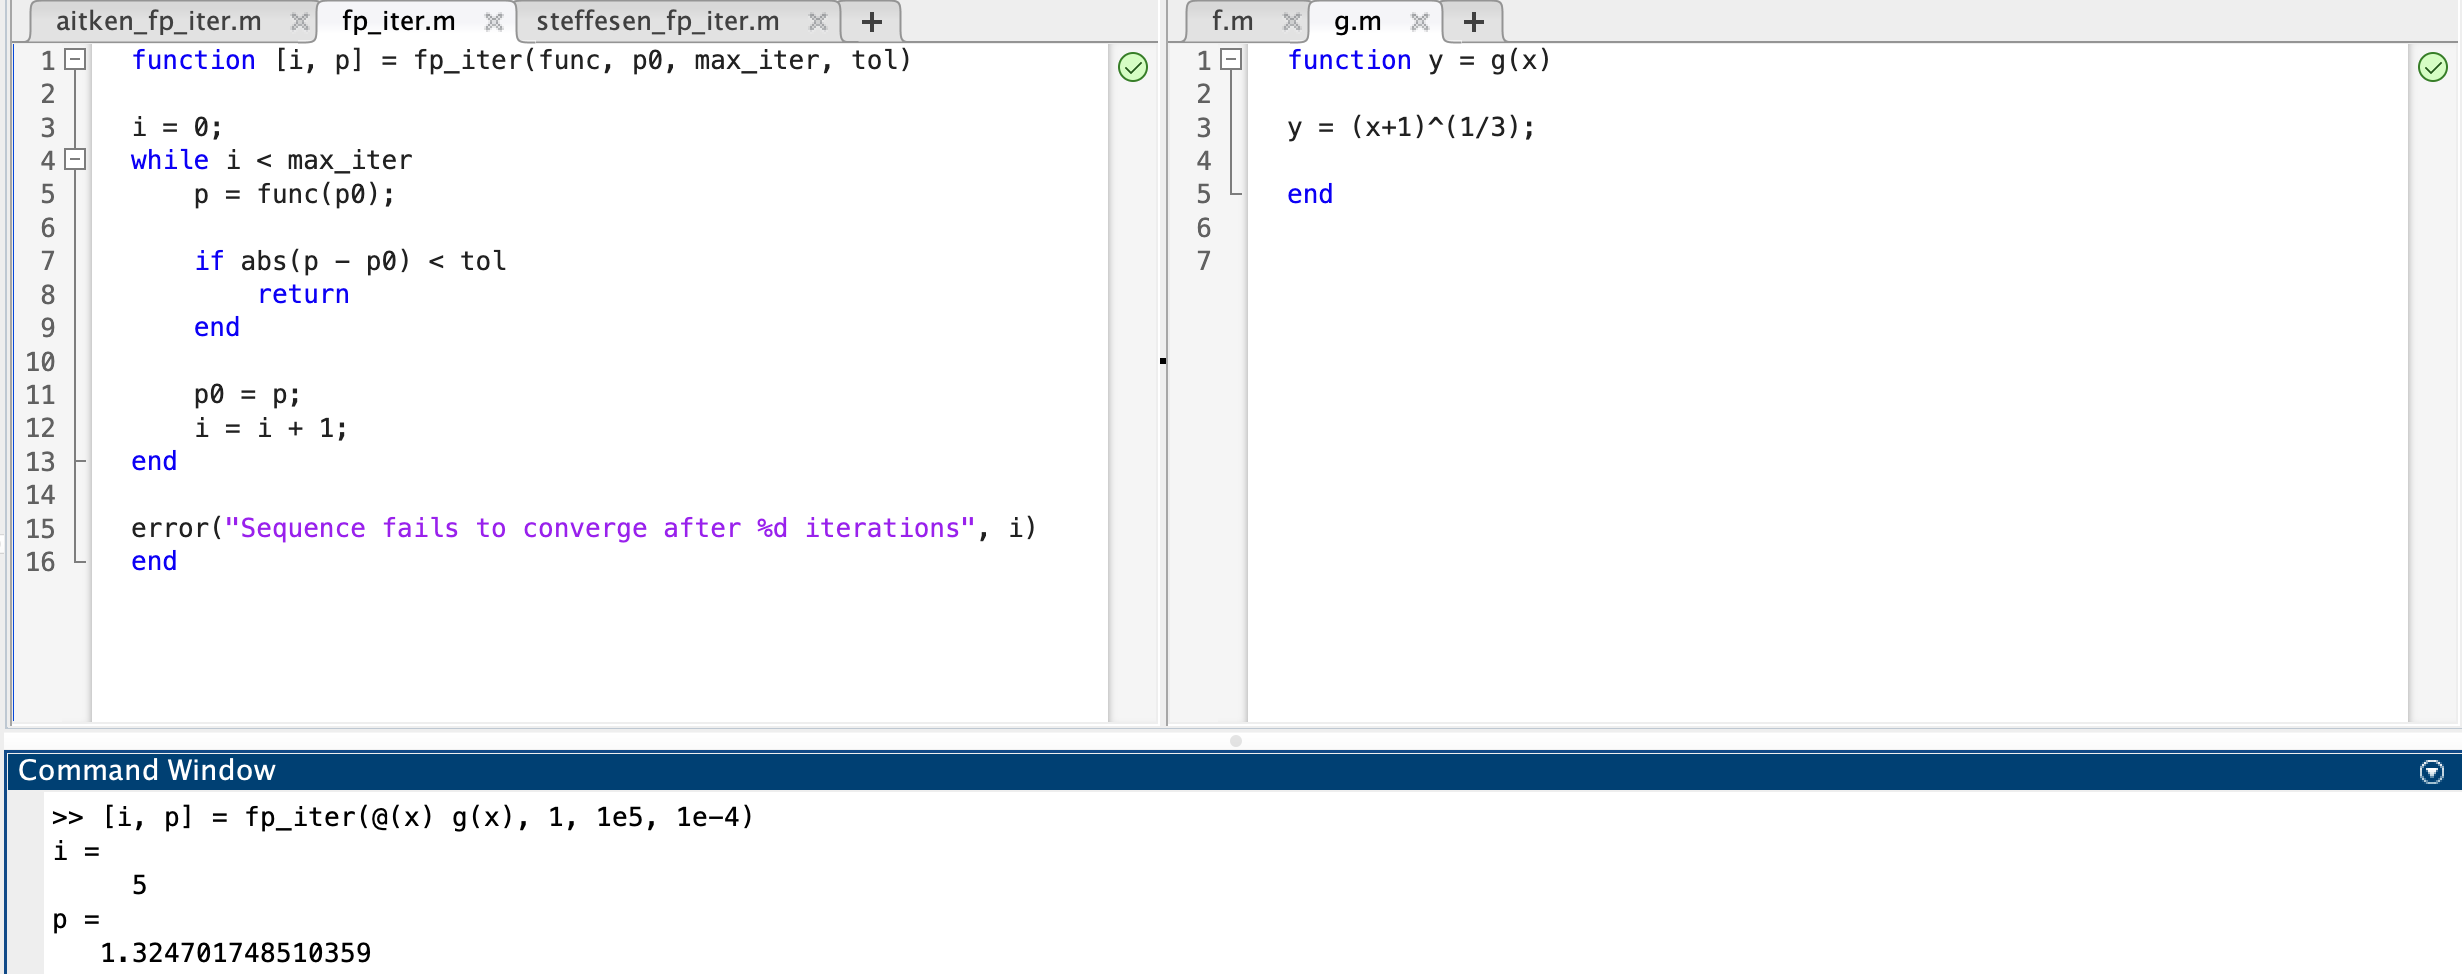
\includegraphics[scale=0.2]{2.5.7_2.png}
        \caption{$p = 1.3247$, iterations = 5}
    \end{figure}

    We re-did Exercise 8 of Section 2.2 up to the same accuracy, but it took only 5 iterations.
\end{proof}

\subsection*{Problem 14}
A sequence $\{p_n\}$ is said to be superlinearly convergent to $p$ if 
$$\lim_{n\to\infty}\frac{|p_{n+1}-p|}{|p_n-p|}=0.$$
\begin{description}
    \item[a.] Show that if $p_n\rightarrow p$ of order $\alpha$ for $\alpha>1$, then $\{p_n\}$ 
    is superlinearly convergence to $p$.
    \begin{proof}
        \begin{align*}
            \lim_{n\rightarrow\infty}\frac{|p_{n+1}-p|}{|p_n-p|} & = 
            \lim_{n\rightarrow\infty}\frac{|p_{n+1}-p|}{|p_n-p|^\alpha}\cdot|p_n-p|^{\alpha-1} \\
            & = \lim_{n\rightarrow\infty}\frac{|p_{n+1}-p|}{|p_n-p|^\alpha}\cdot
            \lim_{n\rightarrow\infty}|p_n-p|^{\alpha-1} \\
            & = C\cdot 0 \\
            & = 0.
        \end{align*}
        
    \end{proof}

    \item[b.] Show that $p_n=\frac{1}{n^n}$ is superlinearly convergent to 0 but does not 
    converge to 0 of order $\alpha$ for any $\alpha>1$.
    \begin{proof}
        \textbf{Superlinear convergence:}
        \begin{align*}
            \lim_{n\rightarrow\infty}\frac{|p_{n+1}-p|}{|p_n-p|} & = 
            \lim_{n\rightarrow\infty}\frac{\frac{1}{(n+1)^{n+1}}}{\frac{1}{n^n}} \\
            & = \lim_{n\rightarrow\infty}\frac{n^n}{(n+1)^{n+1}} \\
            & = \lim_{n\rightarrow\infty}\left(\frac{n}{n+1}\right)^n\cdot\frac{1}{n+1} \\
            & = 0.
        \end{align*}

        \textbf{Not of order $\alpha$ for any $\alpha>1$:} 
        We want to evaluate
        \begin{align}
            \lim_{n\rightarrow\infty}\frac{|p_{n+1}-p|}{|p_n-p|^\alpha} & =
            \lim_{n\rightarrow\infty}\frac{\frac{1}{(n+1)^{n+1}}}{\left(\frac{1}{n^n}\right)^\alpha} \nonumber \\
            & = \lim_{n\rightarrow\infty}\frac{n^{\alpha n}}{(n+1)^{n+1}} \nonumber \\
            & = \lim_{n\rightarrow\infty}\frac{n^{\alpha n}}{n^{n+1}+O(n^{n})} \qquad 
            (\emph{binomial expansion of denominator}) \nonumber \\
            & = \lim_{n\rightarrow\infty}\frac{n^{\alpha n -n-1}}{1+O\left(\frac{1}{n}\right)}.
        \end{align}
        Now notice 
        \begin{align*}
            \alpha n - n - 1 & = n(\alpha-1)-1 \\
            \lim_{n\rightarrow\infty}\alpha n - n - 1 & = \lim_{n\rightarrow\infty}n(\alpha-1)-1 \\
            & = \infty. \qquad (\emph{if $\alpha>1$})
        \end{align*}
        Therefore, the limit at (1) is $\infty$ and $p_n$ is not of order $\alpha$ for any 
        $\alpha>1$.
    \end{proof}
\end{description}

\subsection*{Problem 15}
Suppose that $\{p_n\}$ is superlinearly convergent to $p$. Show that 
$$\lim_{n\rightarrow\infty}\frac{|p_{n+1}-p_n|}{|p_n-p|}=1.$$
\begin{proof}
    \begin{align*}
        \lim_{n\rightarrow\infty}\frac{|p_{n+1}-p_n|}{|p_n-p|} & \le
        \lim_{n\rightarrow\infty}\frac{|p_{n+1}-p|+|p-p_n|}{|p_n-p|} \\
        & \le \lim_{n\rightarrow\infty}\frac{|p_{n+1}-p|}{|p_n-p|}+
        \lim_{n\rightarrow\infty}\frac{|p-p_n|}{|p_n-p|} \\
        & \le 1.
    \end{align*}
    At the same time, 
    \begin{align*}
        \lim_{n\rightarrow\infty}\frac{|p_{n+1}-p_n|}{|p_n-p|} & =
        \lim_{n\rightarrow\infty}\frac{|(p_{n+1}-p)-(p_n-p)|}{|p_n-p|} \\
        & \ge \lim_{n\rightarrow\infty}\frac{||(p_{n+1}-p)|-|(p_n-p)||}{|p_n-p|} \\
        & \ge \lim_{n\rightarrow\infty}|\frac{|(p_{n+1}-p)|}{|p_n-p|}-\frac{|(p_n-p)|}{|p_n-p|}| \\
        & \ge \lim_{n\rightarrow\infty}|\frac{|(p_{n+1}-p)|}{|p_n-p|}-1| \\
        & \ge |\lim_{n\rightarrow\infty}\frac{|(p_{n+1}-p)|}{|p_n-p|}-1| \\
        & \ge 1.
    \end{align*}

    Therefore, 
    \begin{align*}
        & 1\le\lim_{n\rightarrow\infty}\frac{|p_{n+1}-p_n|}{|p_n-p|}\le 1 \\
        \Rightarrow & \lim_{n\rightarrow\infty}\frac{|p_{n+1}-p_n|}{|p_n-p|}=1.
    \end{align*}
\end{proof}

\newpage
\section*{Section 2.6}
\subsection*{Problem 2be}
Find approximations to within $10^{-5}$ to all the zeros of \textbf{b.} 
$$f(x)=x^4-2x^3-12x^2+16x-40$$ and \textbf{e.} 
$$f(x)=16x^4+88x^3+159x^2+76x-240$$ by first finding the real zeros using Newton's method and then
reducing to polynomials of lower degree to determine any complex zeros.
\begin{enumerate}
    \item[\textbf{b.}]
    \begin{proof}[Solution]\indent
        \begin{figure}[htb!]
            \centering
            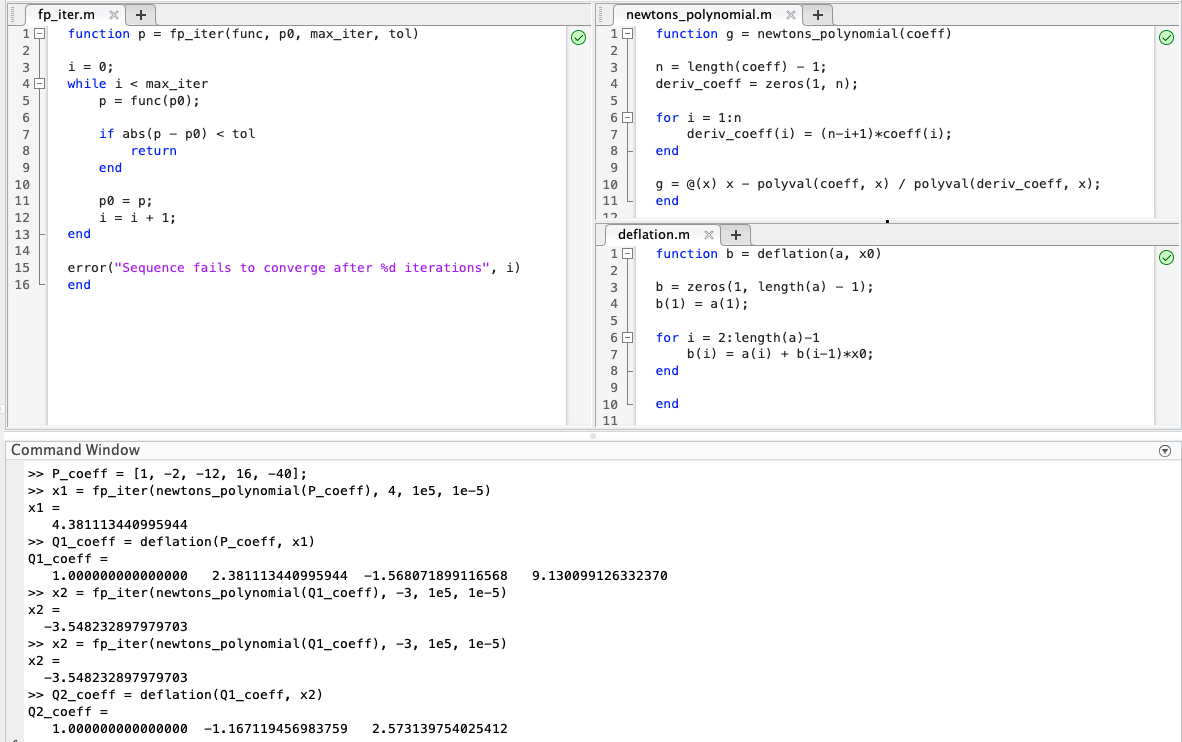
\includegraphics[scale=0.25]{2.6.2b_1.png}
            \caption{$x_1 \approx 4.38111, x_2 \approx -3.54823$}
        \end{figure}
        \begin{figure}[htb!]
            \centering
            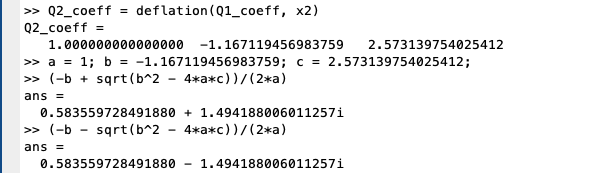
\includegraphics[scale=0.5]{2.6.2b_2.png}
            \caption{$x_3\approx0.58356 + 1.49419i, x_4 \approx 0.58356 - 1.49419i$}
        \end{figure}
        
        \emph{Figure 6:} We first use Newton's method on $f(x)$ to find $x_1$ with starting point at $p_0=4$, and we get 
        $x_1\approx4.38111$. Then we use Horner's method to deflate the polynomial to 
        $$Q_1(x) \approx x^3 + 2.381113x^2 - 1.56807x + 9.1301.$$
        Then, we run Newton's method on $Q_1(x)$ to find $x_2$ with starting point at $p_0=-3$, and 
        we get $x_2\approx-3.54823$. Finally, we use Horner's method to deflate the polynomial to 
        $$Q_2(x) \approx x^2 - 1.16712x + 2.57314.$$
        
        
        \emph{Figure 7:} We solve $Q_2(x)$ by quadratic formula  and get $x_3\approx0.58356 + 1.49419i$ and 
        $x_4 \approx 0.58356 - 1.49419i$.
    \end{proof}

    \item[\textbf{e.}]
    \begin{proof}[Solution]\indent        
        \begin{figure}[htb!]
            \centering
            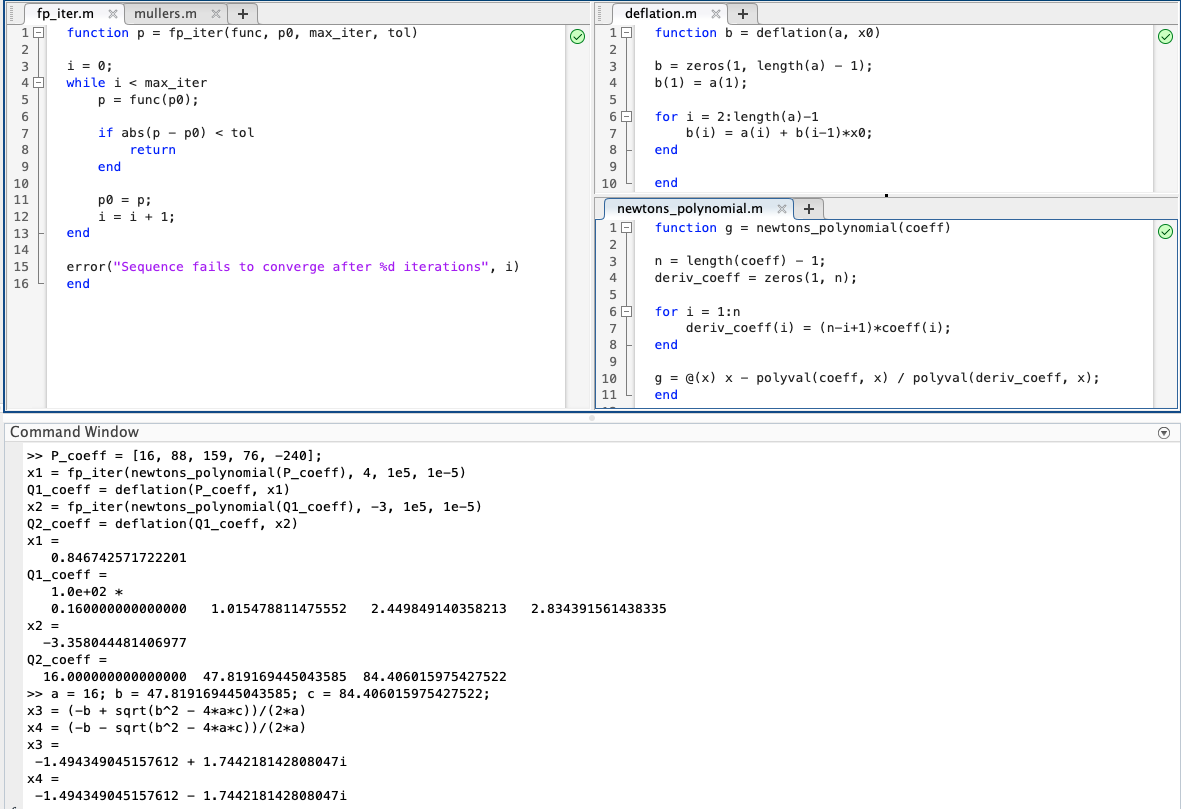
\includegraphics[scale=0.25]{2.6.2e.png}
            \caption{$x_1\approx 0.84674, x_2\approx -3.35804, x_3 \approx -1.49435 + 1.74422i,
            x_4\approx -1.49435 - 1.74422i$}
        \end{figure}

        We followed the exact same procedure from \textbf{b.} to find the zeros of $f(x)$.
    \end{proof}
\end{enumerate}

\newpage
\subsection*{Problem 4be}
Repeat Exercise 2 using Muller's method.
\begin{enumerate}
    \item[\textbf{b.}]
    \begin{proof}[Solution]\indent
        \begin{figure}[htb!]
            \centering
            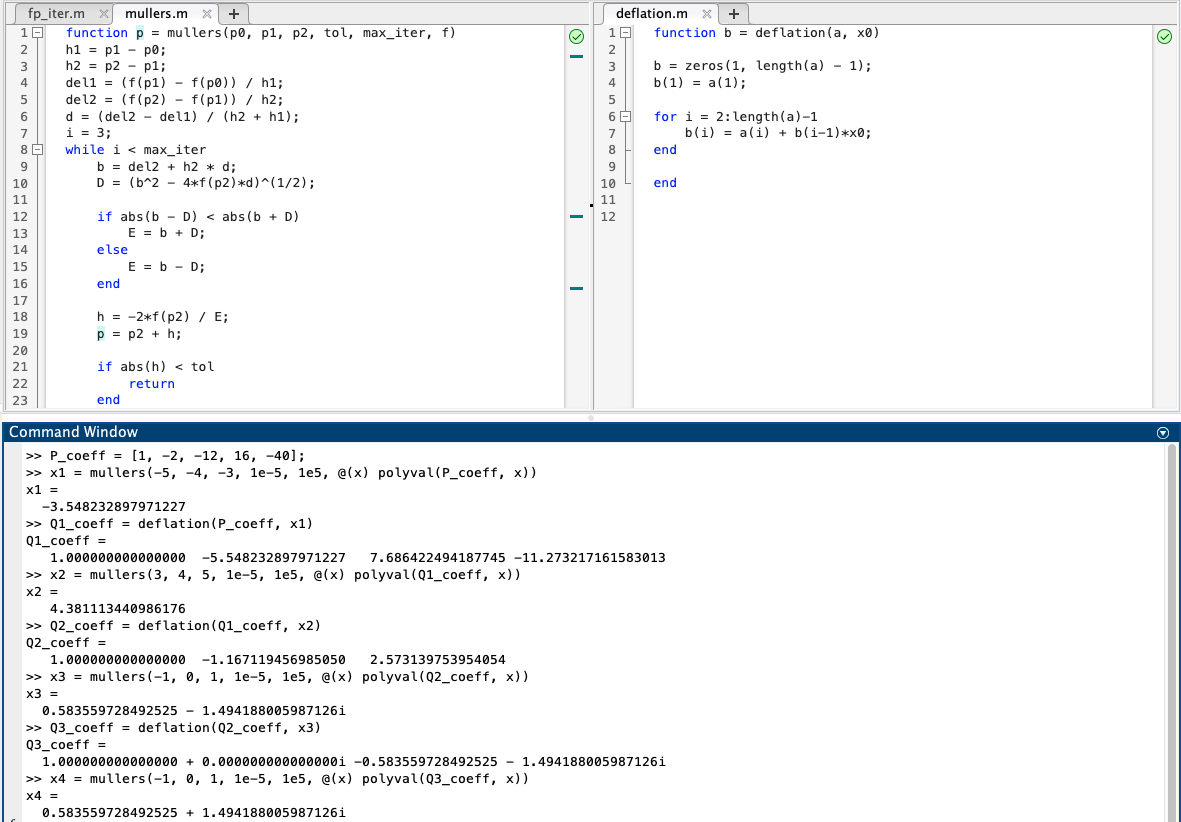
\includegraphics[scale=0.25]{2.6.4b.png}
            \caption{Pretty much same answer as Exercise 2b.}
        \end{figure}

        We use Muller's method to find the first root, then deflate the polynomial. 
        We repeat applying Muller's method on the deflated polynomial until we find all 4 roots.
    \end{proof} 

    \item[\textbf{e.}]
    \begin{proof}[Solution]\indent
        \begin{figure}[htb!]
            \centering
            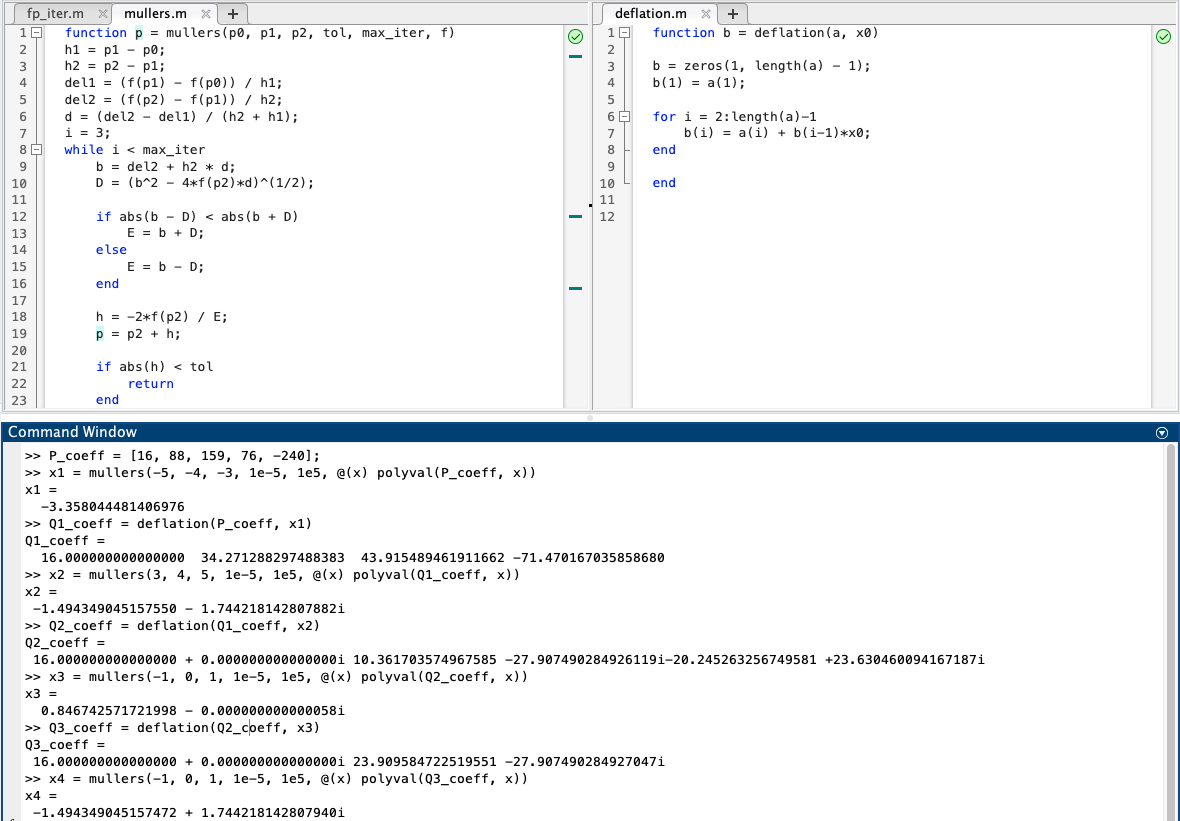
\includegraphics[scale=0.25]{2.6.4e.png}
            \caption{Pretty much same answer as Exercise 2e.}
        \end{figure}
        
        Same procedure as \textbf{b.}
    \end{proof} 
\end{enumerate}

\subsection*{Problem 7abce}
Use each of the following methods to find a solution in $[0.1, 1]$ accurate to within $10^{-4}$ 
for $$600x^4-550x^3+200x^2-20x-1=0.$$
\begin{enumerate*}
    \item[\textbf{a.}] Bisection method 
    \item[\textbf{b.}] Newton's method
    \item[\textbf{c.}] Secant method
    \item[\textbf{e.}] Muller's method
\end{enumerate*}
\begin{enumerate}
    \item[\textbf{a.}]
    \begin{proof}[Solution]\indent
        \begin{figure}[htb!]
            \centering
            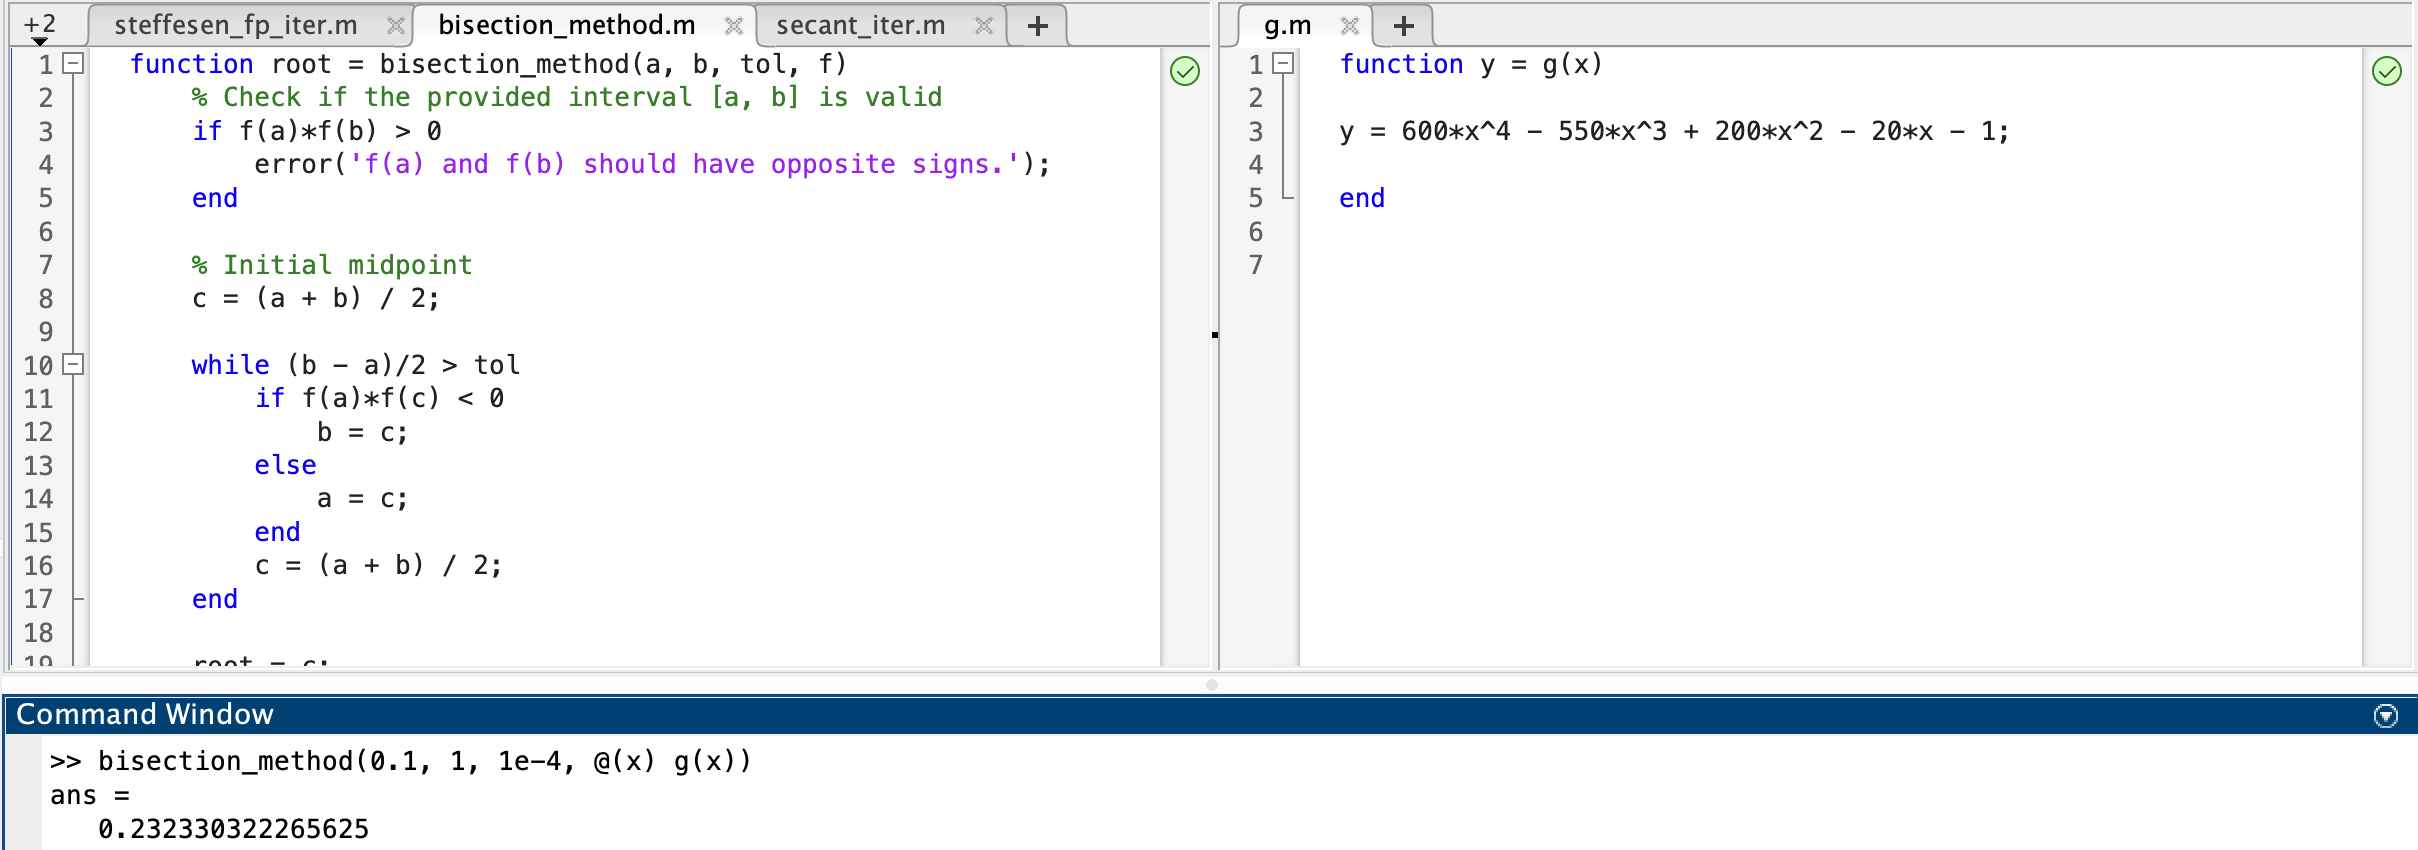
\includegraphics[scale=0.35]{2.6.7a.png}
            \caption{Bisection method}
        \end{figure}
    \end{proof}
    \item[\textbf{b.}]  
    \begin{proof}[Solution]
        \begin{align*}
            f'(x) & = 2400x^3-1650x^2+400x-20 \\
            g(x) & = x-\frac{600x^4-550x^3+200x^2-20x-1}{2400x^3-1650x^2+400x-20}.
        \end{align*}
        \begin{figure}[htb!]
            \centering
            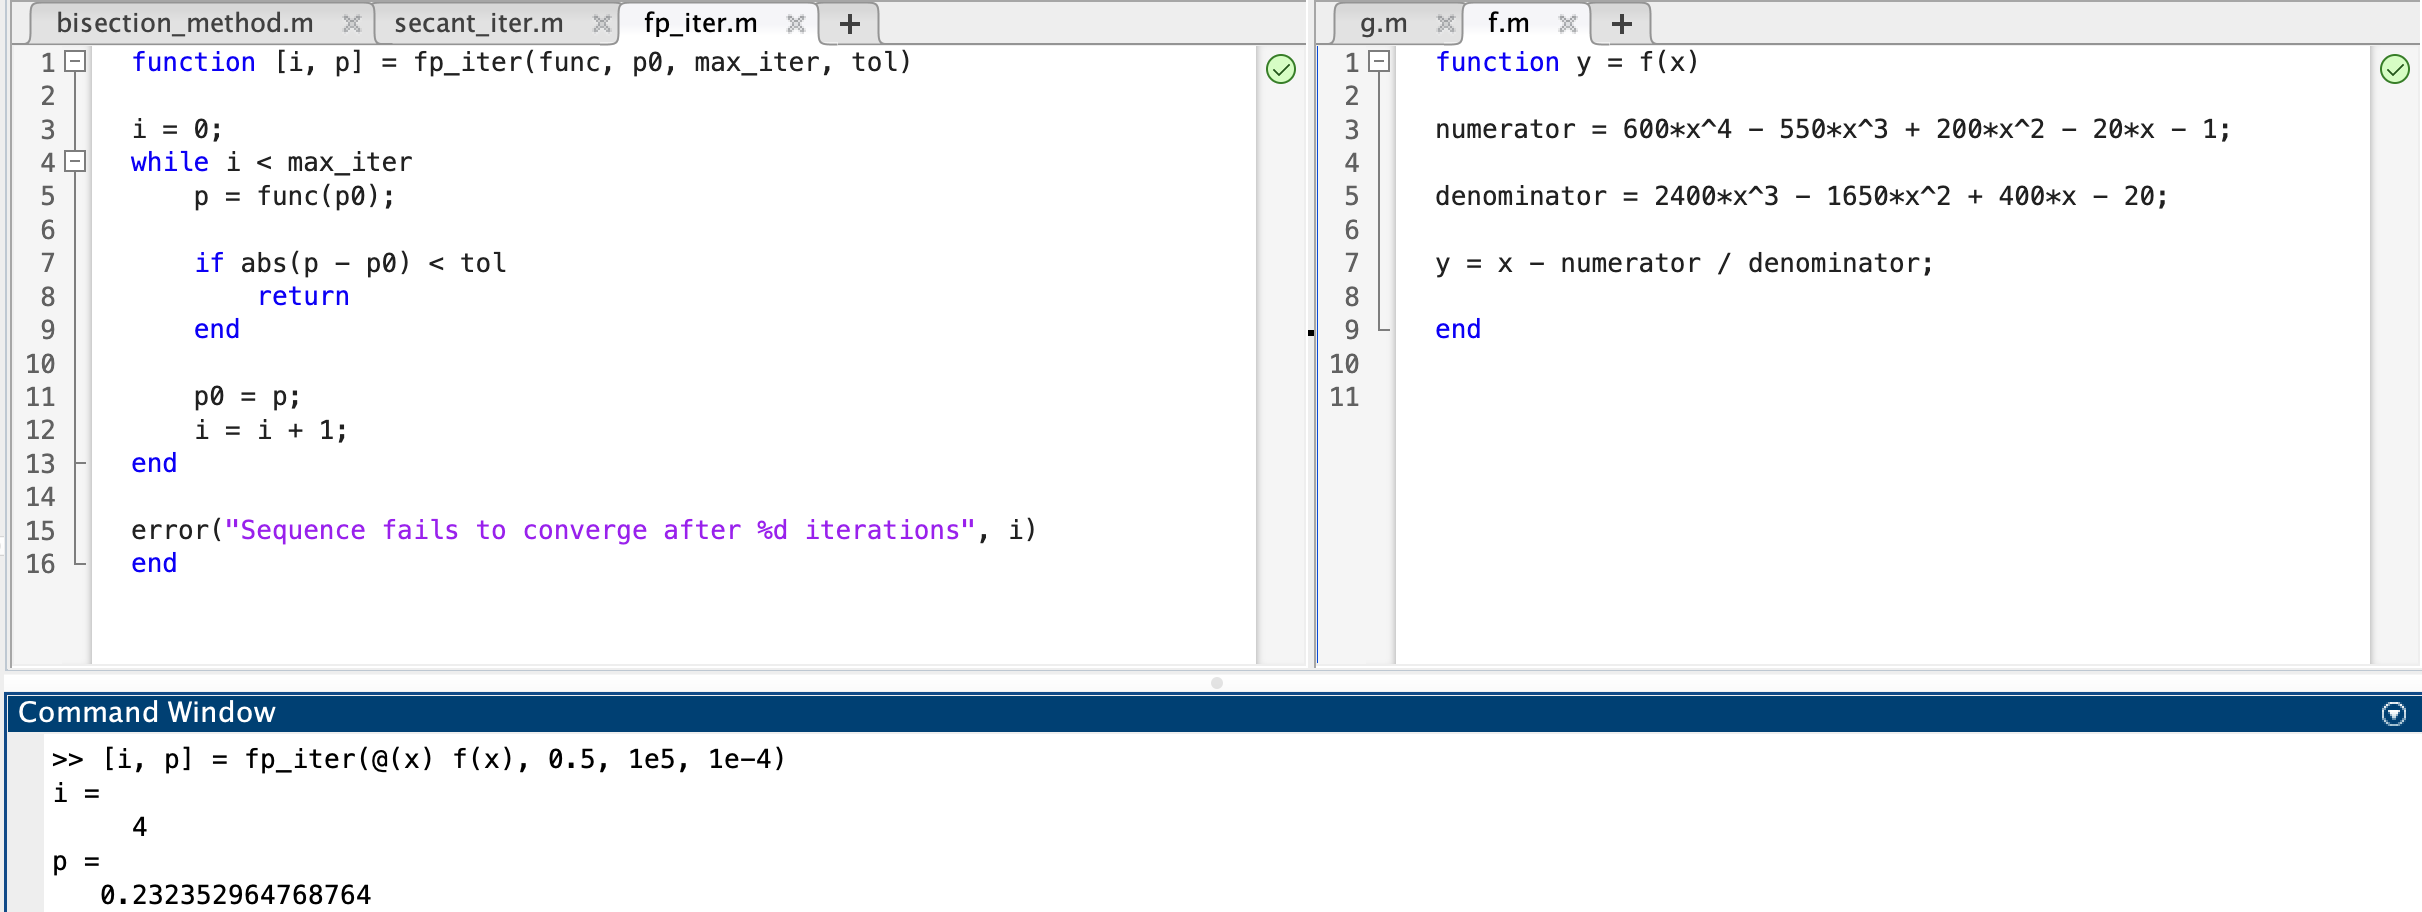
\includegraphics[scale=0.35]{2.6.7b.png}
            \caption{Newton's method}
        \end{figure}
    \end{proof}
    \newpage
    \item[\textbf{c.}]
    \begin{proof}[Solution]\indent
        \begin{figure}[htb!]
            \centering
            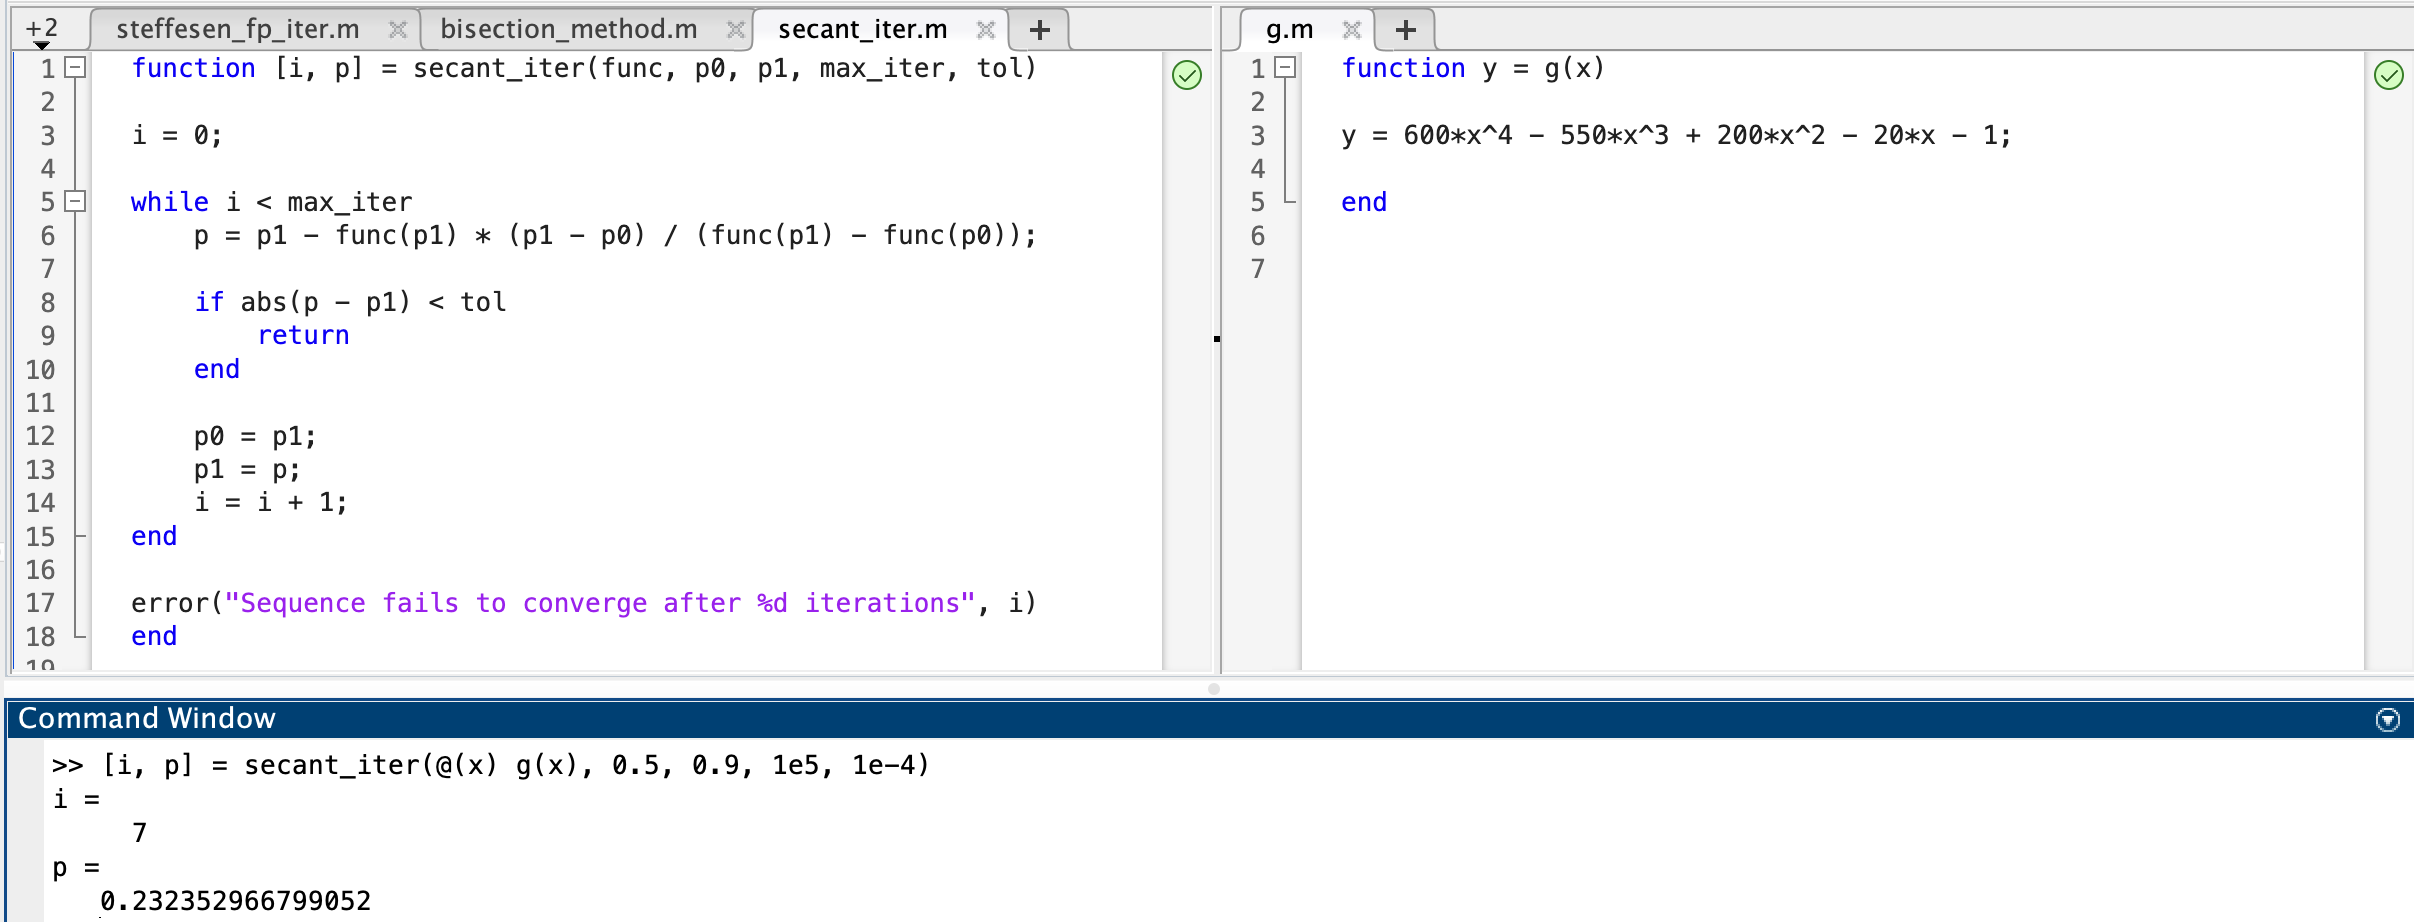
\includegraphics[scale=0.35]{2.6.7c.png}
            \caption{Secant method}
        \end{figure}
    \end{proof}

    \item[\textbf{e.}]
    \begin{proof}[Solution]\indent
        \begin{figure}[htb!]
            \centering
            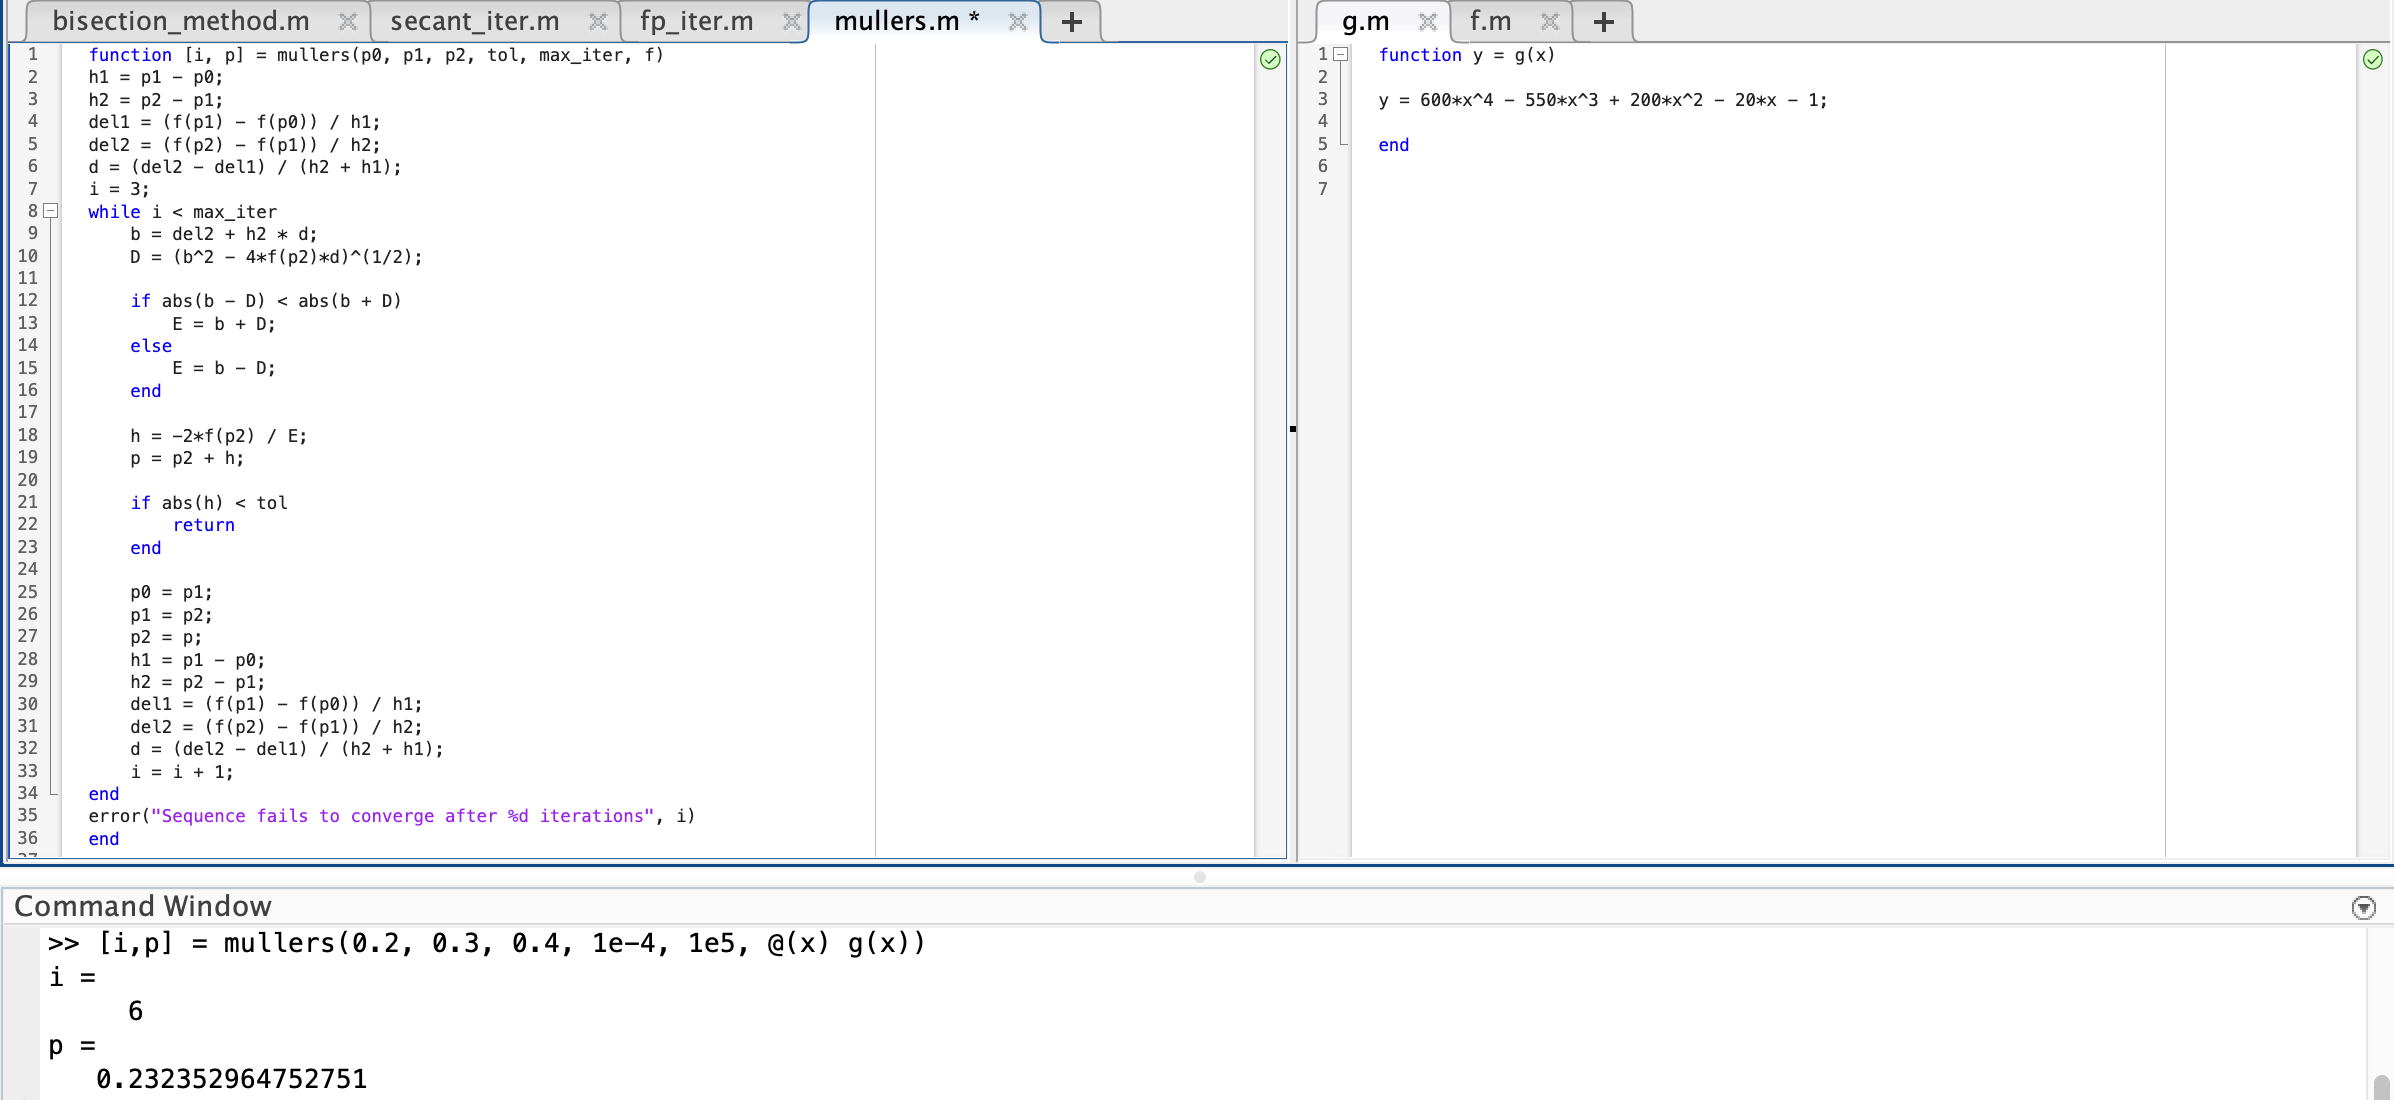
\includegraphics[scale=0.35]{2.6.7e.png}
            \caption{Muller's method}
        \end{figure}
    \end{proof}
    
\end{enumerate}

\newpage
\subsection*{Problem 9}
A can in the shape of a right circular cylinder is to be constructed to contain $1000 cm^3$. 
The circular top and bottom of the can must have a radius of $0.25 cm$ more than the radius of the 
can so that the excess can be used to form a seal with the side. The sheet of material being formed 
into the side of the can must also be $0.25 cm$ longer than the circumference of the can so that a 
seal can be formed. Find, to within $10^{-4}$, the minimal amount of material needed to construct 
the can.
\begin{proof}[Solution]
    We can formulate the problem as 
    \begin{align*}
        \min_{r,h} & \quad f(r, h) = 2\pi (r+0.25)^2+(2\pi r+0.25)h \\
        \text{s.t.} & \quad \pi r^2h=1000.
    \end{align*}

    Notice we can rewrite $f(r,h)$ as 
    \begin{align*}
        f(r) & = 2\pi (r+0.25)^2+(2\pi r+0.25)\frac{1000}{\pi r^2} \\
        & = 2\pi (r+0.25)^2+\frac{2000}{r} \\
        & = 2\pi r^2 + \pi r + 0.125\pi + \frac{2000}{r} + \frac{250}{\pi r^2}.
    \end{align*}
    
    Then, we set $f'(r) = 0$ to find the critical points that will minimize the function.
    \begin{align*}
        f'(r) = 4\pi r + \pi - \frac{2000}{r^2} - \frac{500}{\pi r^3} & = 0 \\
        4\pi r^4 + \pi r^3 - 2000r - \frac{500}{\pi} & = 0.
    \end{align*}
    
    \begin{figure}[htb!]
        \centering
        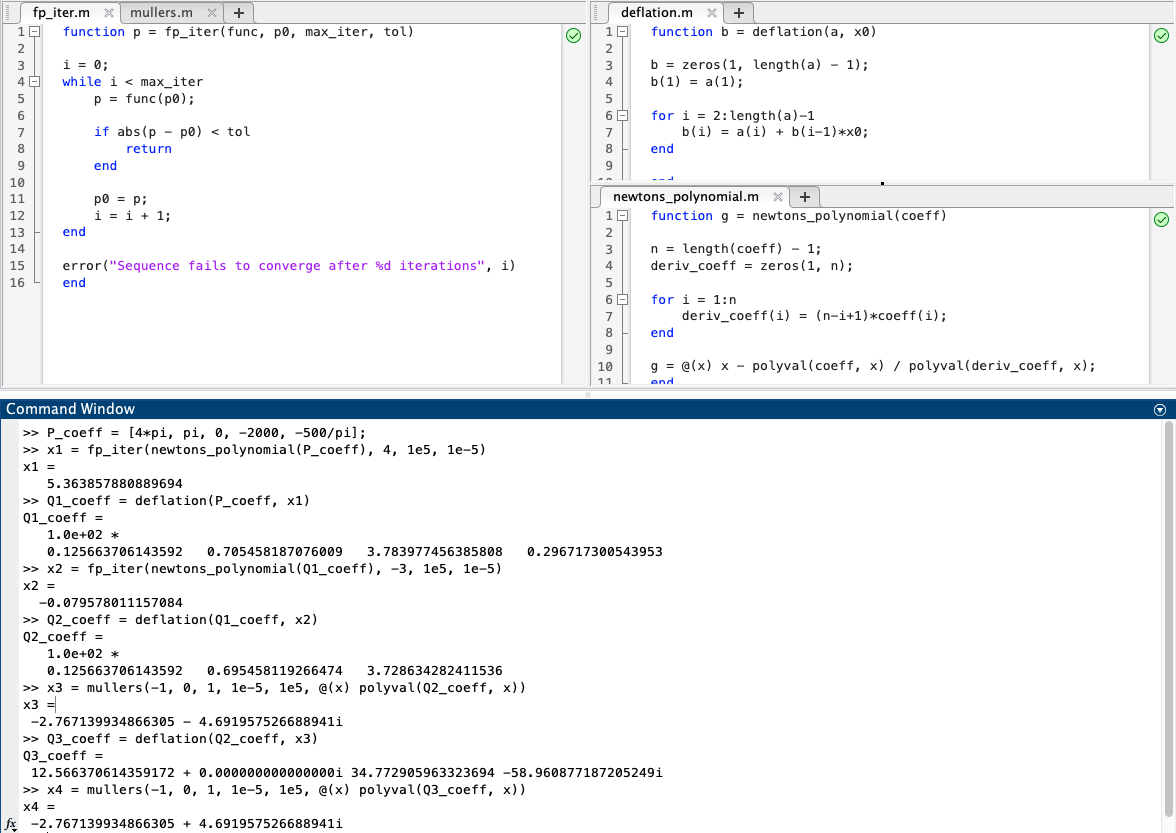
\includegraphics[scale=0.25]{2.6.9_1.png}
        \caption{$r = x_1 \approx 5.36386$}
    \end{figure}

    The only reasonable root being a positive real numer is $r = x_1 \approx 5.36386$. With a few 
    sanity check by pluggin in a few points near $r = 5.36386$ to $f(r)$, indeed 
    $r = 5.36386$ is a local minimum.
    
\end{proof}


\end{document}
